\documentclass[tikz,border=2pt]{standalone}
\usepackage{amsmath,amssymb}
\usepackage{pgfplots}
\pgfplotsset{compat=1.18}

\begin{document}
% The Pois(3) pmf: counts of rare events with mean 3; the mass is spread over all k >= 0 and
% the variance equals the mean.
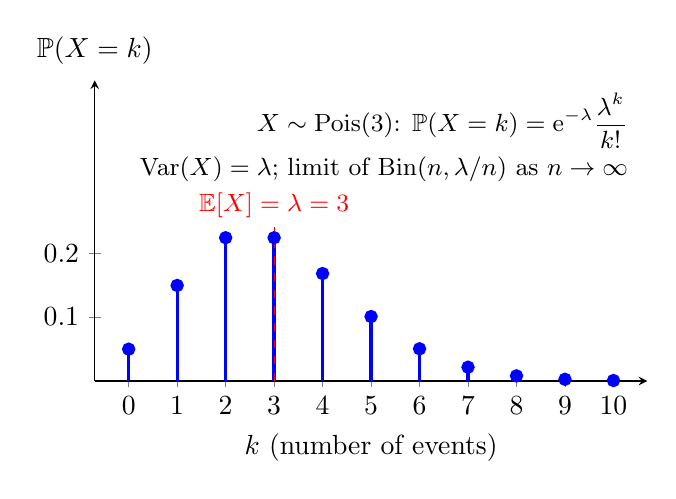
\begin{tikzpicture}
	\begin{axis}[
		axis lines=left, xmin=-0.7, xmax=10.7, ymin=0, ymax=0.47,
		xtick={0,...,10}, ytick={0.1,0.2},
		xlabel={$k$ (number of events)}, ylabel={$\mathbb{P}(X=k)$}, ylabel style={rotate=-90, anchor=south, at={(axis description cs:0,1.02)}},
		width=8.6cm, height=5.4cm, clip=false
		]
		\addplot[ycomb, blue, very thick, mark=*, mark size=1.8pt] coordinates {(0,0.0498) (1,0.1494) (2,0.2240) (3,0.2240) (4,0.1680) (5,0.1008) (6,0.0504) (7,0.0216) (8,0.0081) (9,0.0027) (10,0.0008)};
		\draw[red, dashed] (axis cs:3,0) -- (axis cs:3,0.24);
		\node[red, anchor=south, font=\small] at (axis cs:3,0.24) {$\mathbb{E}[X]=\lambda=3$};
		\node[anchor=north east, font=\small, align=right] at (axis cs:10.5,0.465) {$X\sim\operatorname{Pois}(3)$: $\mathbb{P}(X=k)=\mathrm{e}^{-\lambda}\dfrac{\lambda^k}{k!}$\\[2pt] $\operatorname{Var}(X)=\lambda$; limit of $\operatorname{Bin}(n,\lambda/n)$ as $n\to\infty$};
	\end{axis}
\end{tikzpicture}
\end{document}
